\chapter{Analysis}
Computational models are often to large and complex for traditional method to test, this cause developers of those models unwilling to test their models thorough. Furthermore, computational model developer are often scientist or researchers that don’t have extent knowledge in software engineering or software testing. Due to the different training receive by scientist compared to software developer, the importance of software testing is often overlooked.  \\*
Causal model testing can be a powerful tool to test computational model, but for people don’t have specific knowledge in software engineering, causal model testing can be hard tool to use. Causal model testing requires software testers to integrate the causal model with software model that is being tested, consider the complexity of the computational model being tested can be, it is hard to integrate the test into it for non-software engineer tester. There’s currently a lack of user-friendly way to test computational model with causal model testing, it is possible to integrate behave and cucumber to make this easier for people, by integrate Cucumber tester can use easy to understand language to specify the testing process and behave can read and execute these processes. By combining all these researchers who want to test their computational model can have an easy to access tool to test their software.
\begin{center}
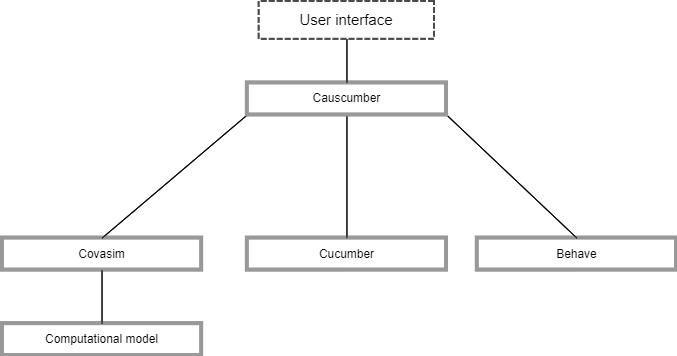
\includegraphics[width=12cm]{figures/Analysis.png}\\
Figure 2. A diagram analysis for the system
\end{center}
\section{Project Requirements}

The main goal of this project is to develop an easy-to-use system where people can use it the execute the feature file they have written, the system will exam the feature file and go through the computational model to check if the model perform as the test specify. As a result, the system should produce a coherent result detailing the accuracy of the tested model. Thus, the systems need to accomplish the following:\\*
1.	As a user, I want this system to be easy to understand, when I use the system, I want to immediate know what I need to do to get the result I want.\\*
2.	As a user, I want the system to go through the feature file I provide and test the computational model with it.\\*
3.	As a user, I want the system to produce a result where I can know the accuracy of the computational model.\\*
Since there’s already a tool been in developing for a while called Causcumber, a modify version of cucumber for testing computational model, what this project aims to accomplish is adding more to this tool. Currently the state of Causcumber is capable of execute some feature files that use to test a computational model named Covasim. And it is capable of returning lot of useful information, but the information still requires some organization to make the result easier to read. And currently there isn’t a way to execute the testing system without using the terminal to execute the command, so there’s a need of a user interface for people to operate the system. Last is that currently the only way to create a feature file is by hand type the files, and this might cause some error or confusion. Therefore, by the end of the project Causcumber should be able to accomplish the following:\\*
1.	As a user, I want the result produce by the system to be clean and easy to understand, focusing on the important part.\\*
2.	As a user, I want to execute and interact with the system through a user interface.\\*
3.	As a user, I want to have a more convenient way to create a feature file, to avoid any mistake during the creation of the feature file.\\*


\section{Ethical, Professional and Legal Issues}

Lorem ipsum dolor sit amet, consectetuer adipiscing elit. Aenean commodo ligula eget dolor. Aenean massa. Cum sociis natoque penatibus et magnis dis parturient montes, nascetur ridiculus mus. Donec quam felis, ultricies nec, pellentesque eu, pretium quis, sem. Nulla consequat massa quis enim. Donec pede justo, fringilla vel, aliquet nec, vulputate eget, arcu. In enim justo, rhoncus ut, imperdiet a, venenatis vitae, justo. Nullam dictum felis eu pede mollis pretium. Integer tincidunt. Cras dapibus. Vivamus elementum semper nisi. Aenean vulputate eleifend tellus. Aenean leo ligula, porttitor eu, consequat vitae, eleifend ac, enim. Aliquam lorem ante, dapibus in, viverra quis, feugiat a, tellus. Phasellus viverra nulla ut metus varius laoreet. Quisque rutrum. Aenean imperdiet. Etiam ultricies nisi vel augue. Curabitur ullamcorper ultricies nisi. Nam eget dui. Etiam rhoncus. Maecenas tempus, tellus eget condimentum rhoncus, sem quam semper libero, sit amet adipiscing sem neque sed ipsum. Nam quam nunc, blandit vel, luctus pulvinar, hendrerit id, lorem. Maecenas nec odio et ante tincidunt tempus. Donec vitae sapien ut libero venenatis faucibus. Nullam quis ante. Etiam sit amet orci eget eros faucibus tincidunt. Duis leo. Sed fringilla mauris sit amet nibh. Donec sodales sagittis magna. Sed consequat, leo eget bibendum sodales, augue velit cursus nunc.
